\chapter{Data integration}
\label{cha:integration}

Ondex front-end is used to visualize networks produced by running an Ondex workflow. 
Originally, the data integration was done by writing a workflow in XML format and by running within the Ondex back-end. 
In the following section, we are going to introduce the Ondex Integrator, which allows users to prepare and run an Ondex workflow using an intuitive GUI 
(for more information see Section \ref{sec:ref_integrator}).
Typically, a simple example for a workflow would be to first select parsers (to import data), then to select mapping methods, 
some filtering methods to improve the quality of the graph and, finally, an export method ({\it{e.g.}}, OXL export for the Ondex file format).


%%%%%%%%%%%%%%%%%%%%%%%%%%%%%%%%%%%%%%%%%%%%%%%%%%%%%%%%%%%%%%%%%%%%%%%%%%%%%%%%%%%%%%%%%%%%%%%%%%%%%%%%%%%%%%%%%%%%%%%%%%%%%%%%%%%%%%%%%%%%%%%%%%%%%%%%%%
\section{Using Ondex Integrator}
\label{sec:integrator}

The Ondex Integrator is available from Tools -$>$ Integrator in the menu of Ondex. 
Figure \ref{fig:integrator} shows it when it first opens up.
For each category showing in the left pane, stable plugins will be displayed by default.
To browse more plugins (when experimental plugins have been selected during installation), 
please untick the option ``Show stable plugins only" in the Configure menu of the Integrator.
As explained above, composing a workflow using the Integrator will require selecting various steps or Ondex plugins -
each of which offer parameters to be set if needed.
N.B.: Grayed out parameters are optional. 

\subsection{Using Ondex Integrator - an Exercise}
\label{sec:integrator_exercise}

\begin{figure}[H]
\centering
\subfigure[Botrytis Cinerea on grape]{
	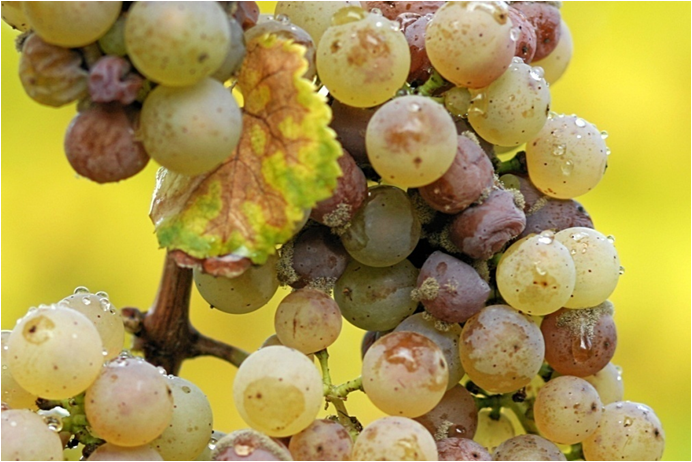
\includegraphics[scale=0.4]{images/Oct12/grape.png} 
	\label{fig:grape}
}
\subfigure[Botrytis Cinerea on strawberry]{
	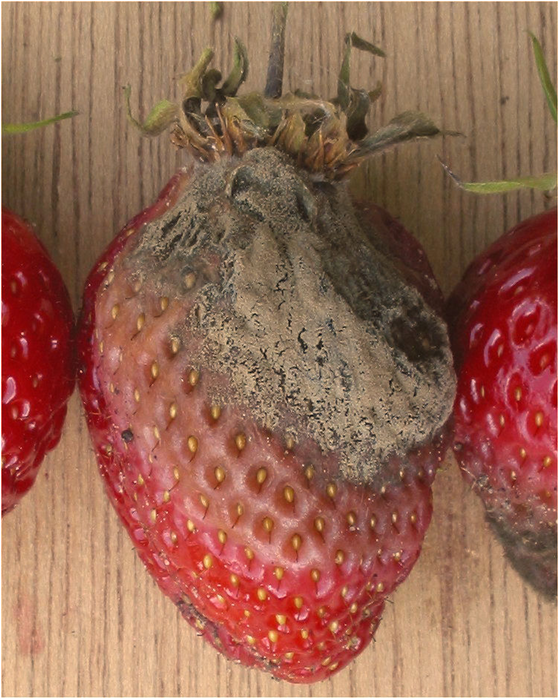
\includegraphics[scale=0.4]{images/Oct12/strawberry.png} 
	\label{fig:strawberry}
}
\label{fig:bot_in_action}
\caption{Botrytis Cinerea}
\end{figure}

\textit{Botrytis cinerea} (\url{http://www.broad.mit.edu/annotation/genome/botrytis_cinerea/}) is a necrotrophic fungus that affects many plant species. 
Its most notable hosts are wine grapes (see Figure \ref{fig:grape}) and strawberries (see Figure\ref{fig:strawberry}). 
Genomic data are available for this fungus, however we do not have much phenotypic data related to genes.
The PHI-base database (\url{http://www.phi-base.org/}) is a reference database of virulence and pathogenicity genes validated by gene disruption experiments. 
It contains information on experimentally verified pathogenicity, virulence and effector genes from bacterial, 
fungal and Oomycete pathogens identified from the scientific literature. 

For this example, techniques of comparative genomics were combined with data integration methods to predict pathogenicity genes in pathogenic organisms. 
The InParanoid algorithm\footnote{Remm M., Storm C.E., Sonnhammer E.L. (2001). 
``Automatic clustering of orthologs and in-paralogs from pairwise species comparisons''. Journal of Molecular Biology, 314(5):1041-52, PubMed ID: 11743721.}
was implemented as part of the Ondex system for the prediction of orthologous groups of proteins.
The workflow we are working on in this section is illustrated in Figure \ref{fig:phi_bot}.

\begin{figure}[H]
\centering
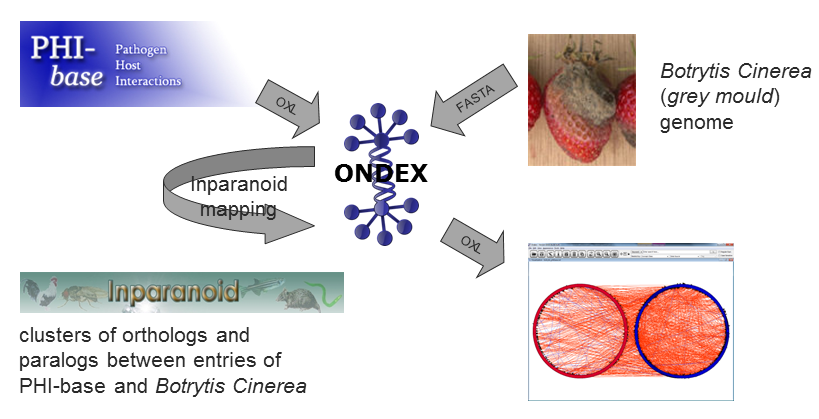
\includegraphics[scale=0.5]{images/Oct12/integration_phi_bot.png} 
\caption{Integrating PHI-base and genomic information of \textit{Botrytis Cinerea}}
\label{fig:phi_bot}
\end{figure}


\begin{figure}[H]
\centering
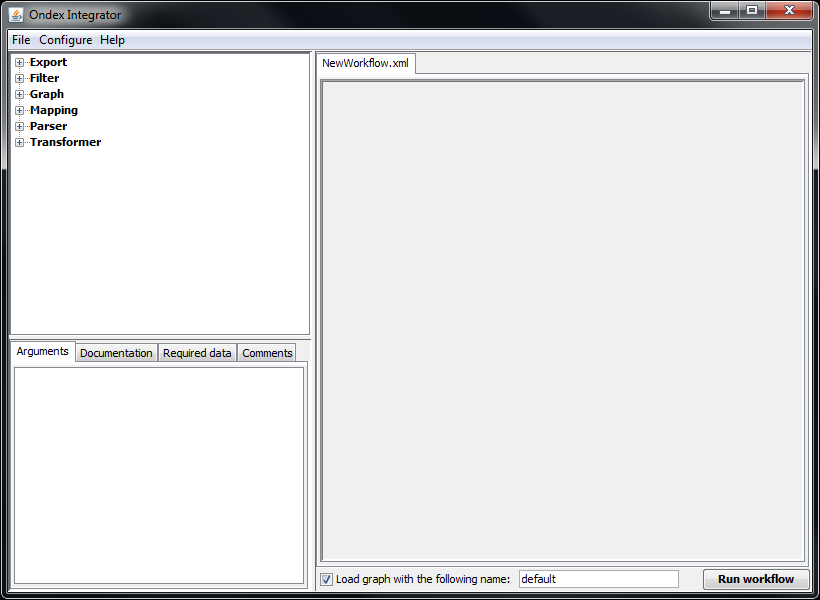
\includegraphics[scale=0.5]{images/Oct12/integrator.png} 
\caption{Data integration using the graphical interface - Ondex Integrator}
\label{fig:integrator}
\end{figure}


Note: Running this workflow with the whole genome sequence from \textit{Botrytis} will take about an hour. 
If you wish to see quick results during this hands-on tutorial, we suggest you use a FASTA file which has been prepared for this purpose: 
short.fasta which can be found under Tutorial\_files/Data\_integration/Integrator. 
This file contains a tenth of the entire genome and will take about 3 minutes. 
The results show a smaller graph which can be analysed nevertheless. 
In Chapter \ref{cha:comp}, we will load up the results for the whole genome and study them using
Ondex annotators (these results are saved under Tutorial\_files/Application\_cases/botrytis\_phibase.oxl).

Note: Before running a workflow in the Ondex Integrator, make sure you save your current workflow 
so you can re-open it as you might not get all the parameters right the first time around.
For this example, the steps needed in the workflow are as follows
({\em{All the files needed here are saved under Tutorial\_files/Data\_integration/Integrator}}):

\begin{itemize}
\item Parsing the file containing the PHI-base database (Parser - OXL Parser, see Figure \ref{fig:integrator_oxlimport}). 
Note: A ``New memory graph'' pre-step is automatically loaded.
\begin{figure}[H]
\centering
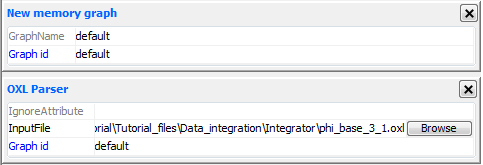
\includegraphics[scale=0.6]{images/Oct12/oxlimport.png} 
\caption{Parser - OXL Parser}
\label{fig:integrator_oxlimport}
\end{figure}
Opening this OXL file directly would produce the metagraph shown in Figure \ref{fig:metagraph_phibase}.
\begin{figure}[H]
\centering
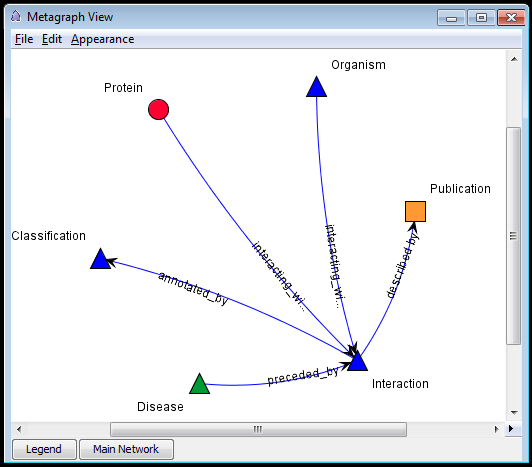
\includegraphics[scale=0.6]{images/Oct12/phibase.png} 
\caption{Metagraph - PHI-base}
\label{fig:metagraph_phibase}
\end{figure}
If you have time, have a look at the main graph. 
In particular, try to find which concepts hold the phenotypic information we are actually interested in for this workflow.
This will later determine which concept classes you can filter out, which ones you should keep and/or combine.

\item Parsing the file downloaded from the Broad institute website for the sequence of \textit{Botrytis Cinerea} 
(Parser - FASTA file parser, see Figure \ref{fig:integrator_fasta})
Note: The taxonomy ID for \textit{Botrytis Cinerea} was found on \url{http://www.ncbi.nlm.nih.gov/taxonomy/} (40559). 
CC stands for Concept Class and is therefore ``Protein''. 
SeqType stands for Sequence Type and is in this case ``AA'', amino acid.
\begin{figure}[H]
\centering
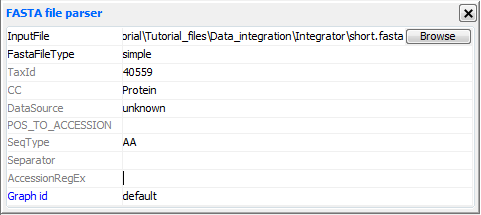
\includegraphics[scale=0.6]{images/Oct12/fasta.png} 
\caption{Parser - FASTA file parser}
\label{fig:integrator_fasta}
\end{figure}
An export (select Export in the left-hand information tree and OXL Export in the list of exporters) at the end of a workflow
containing only the FASTA file parser would produce the metagraph shown in Figure \ref{fig:metagraph_botrytis}.
\begin{figure}[H]
\centering
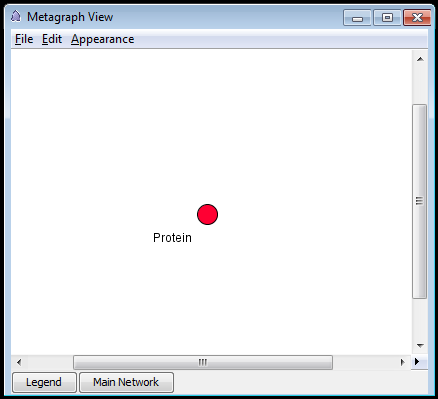
\includegraphics[scale=0.6]{images/Oct12/botrytis.png} 
\caption{Metagraph - Botrytis}
\label{fig:metagraph_botrytis}
\end{figure}

\item After parsing the two data sources, they are mapped to each other using the ``Inparanoid'' mapping which uses pair-wise sequence alignment results 
generated by BLAST \url{http://www.ncbi.nlm.nih.gov/books/NBK1762/} (Mapping - Inparanoid, see Figure \ref{fig:integrator_inparanoid}). 
The ``Evalue'' parameter is passed on to BLAST.
``Cutoff'' and ``Overlap'' are post filter parameters which specify a bit score cutoff and the minimum length of the match compared to the longest sequence.
({\em{If BLAST is not installed on your machine, please download the appropriate installer from 
\url{ftp://ftp.ncbi.nlm.nih.gov/blast/executables/blast+/LATEST/} 
The Inparanoid mapping method expects to be given the bin directory of your BLAST installation.}})
\begin{figure}[H]
\centering
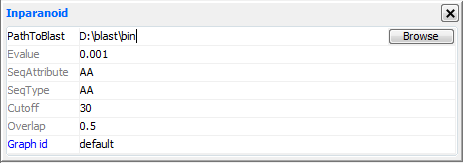
\includegraphics[scale=0.6]{images/Oct12/inparanoid.png} 
\caption{Mapping - Inparanoid}
\label{fig:integrator_inparanoid}
\end{figure}
An export at this stage would produce the metagraph shown in Figure \ref{fig:inparanoid_results}.
\begin{figure}[H]
\centering
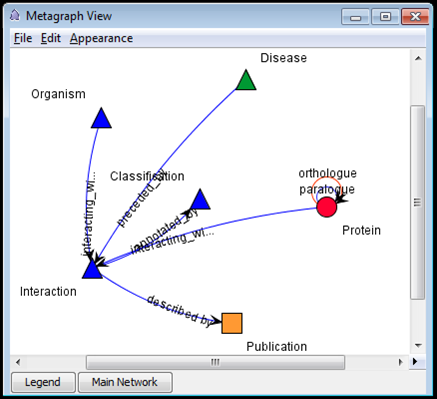
\includegraphics[scale=0.6]{images/Oct12/inparanoid_results.png} 
\caption{Metagraph - Results of the Inparanoid mapping method}
\label{fig:inparanoid_results}
\end{figure}

\item To reduce the complexity of the network several concept classes we are not interested in are filtered out
(Filter - ConceptClass Filter, see Figure \ref{fig:integrator_cc}).
\begin{figure}[H]
\centering
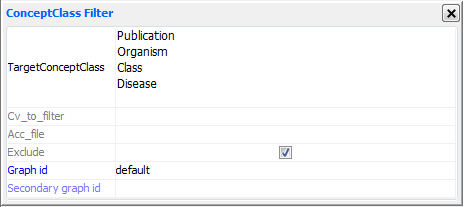
\includegraphics[scale=0.6]{images/Oct12/cc.png} 
\caption{Filter - ConceptClass Filter}
\label{fig:integrator_cc}
\end{figure}

\item In PHI-base a concept of class ``Protein'' is always linked to an ``Interaction'' which carries the specific phenotype. 
To merge both information from ``Protein'' and ``Interaction'' the relation type ``int\_w'' is collapsed and 
the connected concepts are merged into a single concept of concept class ``Interaction:Protein''. 
(Transformer - Relation Collapser, see Figure \ref{fig:integrator_relationCollapser})
\begin{figure}[H]
\centering
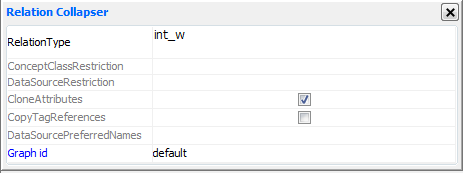
\includegraphics[scale=0.6]{images/Oct12/relationCollapser.png} 
\caption{Transformer - Relation Collapser}
\label{fig:integrator_relationCollapser}
\end{figure}
An export at this stage would produce the metagraph shown in Figure \ref{fig:intermediate_results}.
\begin{figure}[H]
\centering
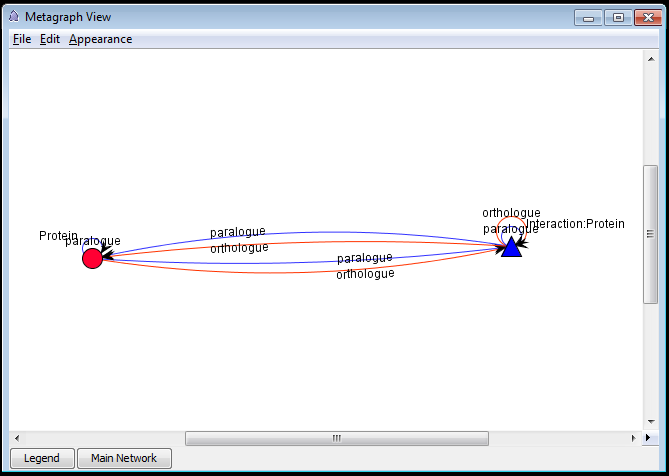
\includegraphics[scale=0.6]{images/Oct12/intermediate_results.png} 
\caption{Metagraph - Results of the ConceptClass Filter and the Relation Collapser}
\label{fig:intermediate_results}
\end{figure}

\item An export at this stage would produce the graph shown in Figure \ref{fig:need_unconnected}.
\begin{figure}[H]
\centering
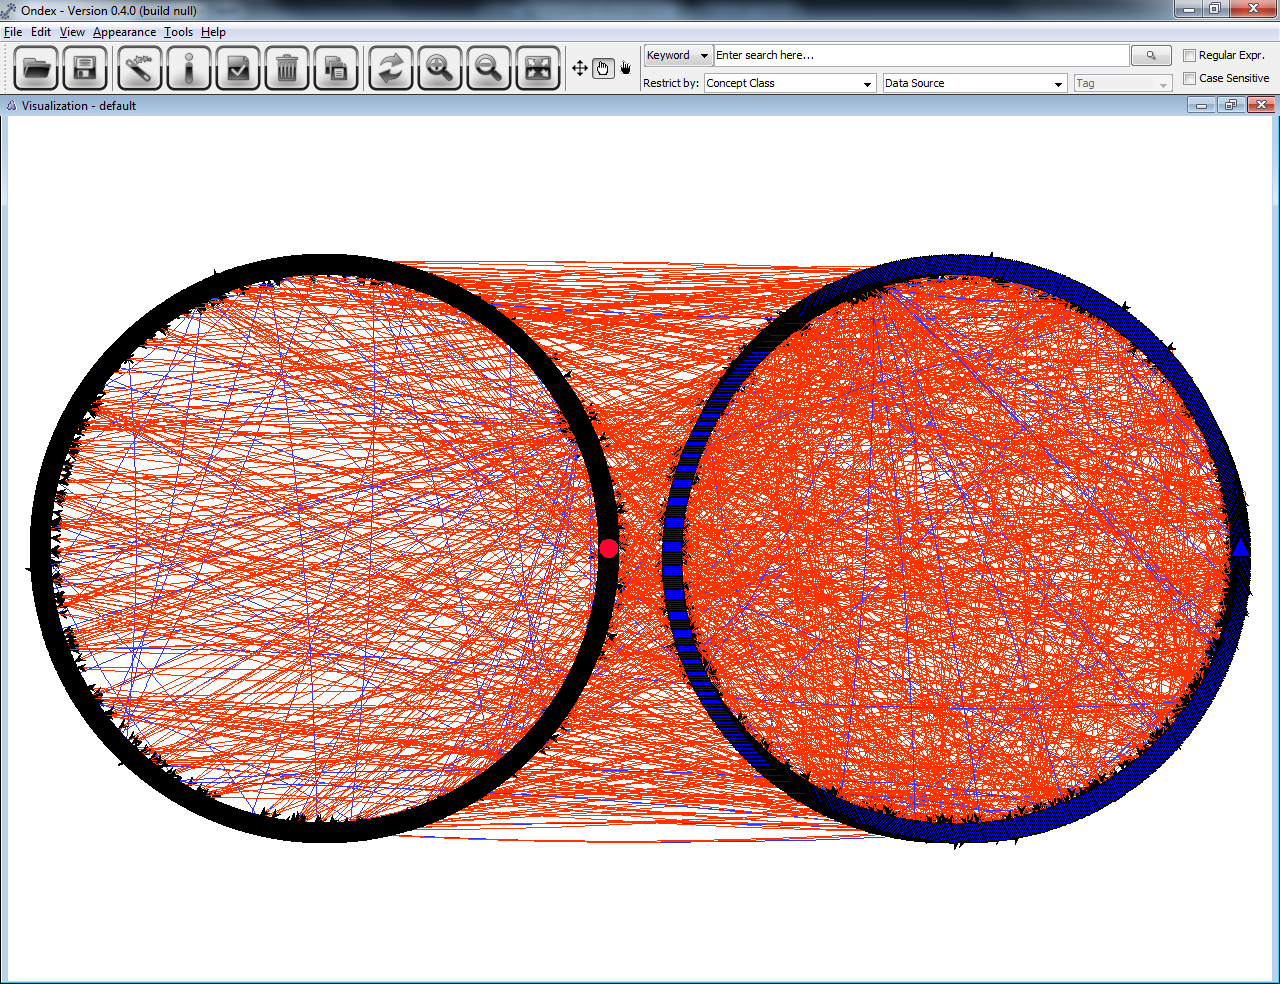
\includegraphics[scale=0.3]{images/Oct12/need_unconnected.png} 
\caption{Main graph - Need for the Unconnected Filter}
\label{fig:need_unconnected}
\end{figure}
The Unconnected Filter is used to remove any isolated concepts (i.e. without any relations to the rest of the network).
(Filter - Unconnected Filter, see Figure \ref{fig:integrator_unconnected})
\begin{figure}[H]
\centering
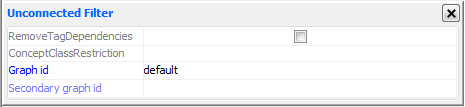
\includegraphics[scale=0.6]{images/Oct12/unconnected.png} 
\caption{Filter - Unconnected Filter}
\label{fig:integrator_unconnected}
\end{figure}

\item An export at this stage would contain the graphs shown in Figure \ref{fig:clusters}.
\begin{figure}[H]
\centering
\subfigure[Main graph - Example of a cluster of interest]{
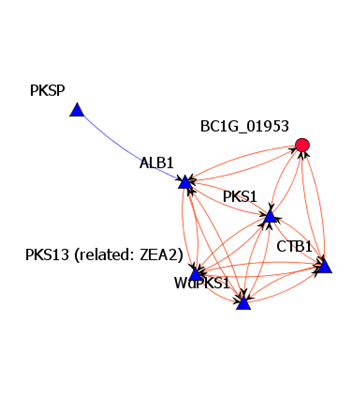
\includegraphics[scale=0.6]{images/Oct12/need_clusters_good.png} 
\label{fig:cluster_good}
}
\subfigure[Main graph - Example of a cluster we wish to remove]{
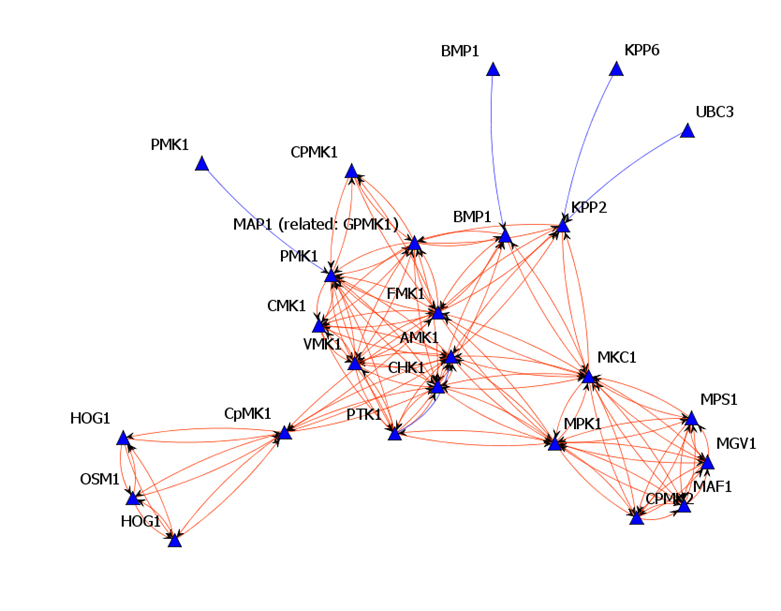
\includegraphics[scale=0.6]{images/Oct12/need_clusters_bad.png} 
\label{fig:cluster_bad}
}
\label{fig:clusters}
\caption{Two kinds of resulting clusters}
\end{figure}
Therefore the next step will only keep clusters of concepts in the network which contain at least one concept of concept class ``Protein'' 
from \textit{Botrytis Cinerea}. 
(Filter - IsolateClusters Filter, available in the experimental package - please untick the option in the Configure menu of the Ondex Integrator,
see Figure \ref{fig:integrator_isolateclusters})
\begin{figure}[H]
\centering
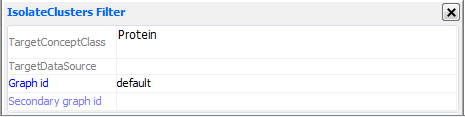
\includegraphics[scale=0.6]{images/Oct12/isolateclusters.png} 
\caption{Filter - Isolateclusters}
\label{fig:integrator_isolateclusters}
\end{figure}

\item The resulting network is exported as OXL (Export - OXL Export, see Figure \ref{fig:integrator_oxlexport}) to an Ondex network file called short\_botrytis\_results.oxl
\begin{figure}[H]
\centering
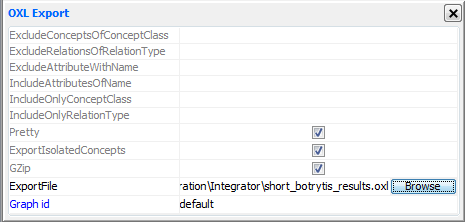
\includegraphics[scale=0.6]{images/Oct12/oxlexport.png} 
\caption{Export - OXL Export}
\label{fig:integrator_oxlexport}
\end{figure}

\end{itemize}
Loading short\_botrytis\_results.oxl in Ondex will look similar to Figure \ref{fig:phi_bot_results}.
\begin{figure}[h]
\centering
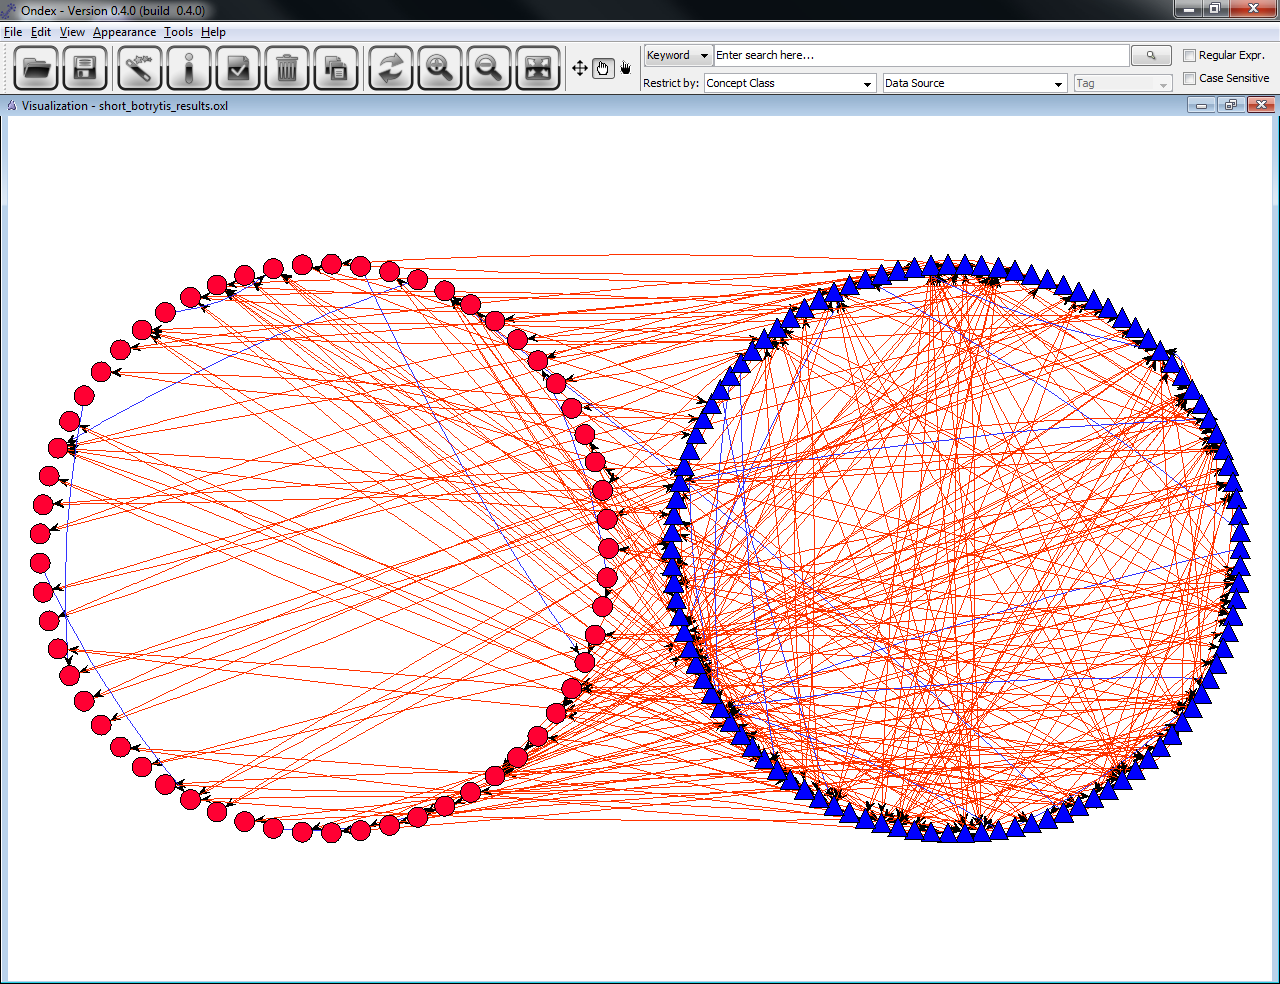
\includegraphics[scale=0.3]{images/Oct12/short_botrytis_results.png} 
\caption{Resulting graph after integration}
\label{fig:phi_bot_results}
\end{figure}




%%%%%%%%%%%%%%%%%%%%%%%%%%%%%%%%%%%%%%%%%%%%%%%%%%%%%%%%%%%%%%%%%%%%%%%%%%%%%%%%%%%%%%%%%%%%%%%%%%%%%%%%%%%%%%%%%%%%%%%%%%%%%%%%%%%%%%%%%%%%%%%%%%%%%%%%%%
\section{Using the scripting console}
\label{sec:parsing_tabdel}
When Ondex does not provide any specific parser for the data a user is interested and this data is in a tab delimited format, 
it is possible to use a general tab delimited parser. This section explains how to use it.

\subsection{Basic functionality and parsing of delimited files}
The prototype based parsing API aims to simplify and speed up the import of user defined formats into Ondex graphs. 
As custom formats are highly variable it is impossible to write a universal parser to deal with all of the possible options. 
This approach aims to provide the middle ground way that retains all of the flexibility but takes care of the complexity involved 
with using the Ondex JAVA API directly. Most delimited files can be parsed in about 5 lines. 
The following guide is primarily for using the API through the scripting interface, although it can be used directly from JAVA as well.

Steps for example 1 (explained below):
\begin{itemize}
\item Open a new empty graph
\item Tools -$>$ Console
\item Type commands in the console or copy and paste the prepared script available at Tutorial\_files/Data\_integration/Console/readme\_scripting.txt
(change the path to test.tab so that it points to the correct file, make sure to keep forward slashes)
\item Press enter (a quarter of a concept should appear in the top-left corner)
\item Appearance -$>$ Layouts -$>$ Gem
\end{itemize}

\textbf{Example 1}
The tab-delimited file in Figure \ref{fig:tab_and_graph} produces the network on its right-hand side (using the commands underneath).
\begin{figure}[h]
\centering
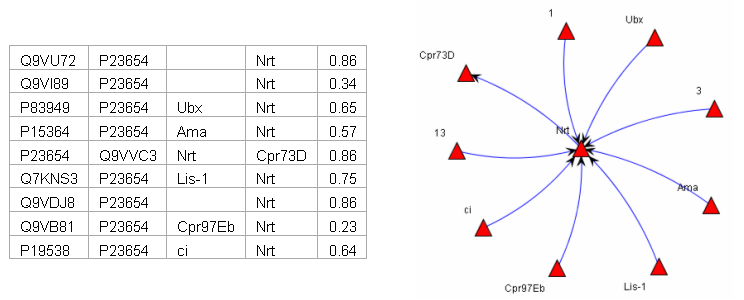
\includegraphics[scale=0.5]{images/Oct12/tab_and_graph.png} 
\caption{Tab-delimited file and generated graph}
\label{fig:tab_and_graph}
\end{figure}


\begin{verbatim}
p = new PathParser(getActiveGraph(), 
	new DelimitedFileReader("C:/test.tab", "	"));
\end{verbatim}
This statement creates a new parser. The ``getActiveGraph()'' method call gives the reference to the last active visualisation frame in Ondex (at least one must be open). 
The ``DelimitedFileReader" takes a path to the file and a delimiter (in this case tab) as an argument.
\begin{verbatim}
c1 = p.newConceptPrototype(
	defAccession(0, "UNIPROTKB"), defCC("Protein"), defName(2));
c2 = p.newConceptPrototype(
	defAccession(1, "UNIPROTKB"), defCC("Protein"), defName(3));
\end{verbatim}
Here new concept prototypes are added to the parser. This method can take any number of arguments in any order. 
The arguments specify which user data (or which column) will be converted to which argument. 
In the above example, the integers 0, 1, 2, 3 represent the number of the column where the information can be found.
\begin{verbatim}
p.newRelationPrototype(
	c1, c2, defAttribute(4, "P-value", "NUMBER"));
\end{verbatim}
This statement creates a relation prototype that will create a relation between the two concepts created from the prototypes ``c1'' and ``c2''. 
The source and target concepts are the only two required arguments. There can be any number of relation attribute arguments that can be in any order.
Attributes get specified using ``defAttribute''.
\begin{verbatim}
p.parse();
\end{verbatim}
Parses the file and creates the graph.

\vspace{1cm}
\textbf{Example 2}
\begin{verbatim}
p = new PathParser(getActiveGraph(), new DelimitedFileReader
("D:/workspace/core/data/importdata/Uniprot2AGI.tab", "	"));
p.newConceptPrototype(defCC("Protein"), 
	defAccession(0, "UNIPROTKB"), defAccession(1, "TAIR"));
p.setProcessingOptions();
\end{verbatim}
Sets the processing options to none - by default the concepts created will always be merged on accessions, 
but the parsing process will take much longer - even if no concepts actually satisfy this requirement.
\begin{verbatim}
p.parse();
\end{verbatim}

\textbf{Attribute specification arguments}
All attribute specification arguments are optional and can be supplied in any order. 
The type of the argument corresponds to the name of the function and the first argument is always either a position in the data vector 
(\textit{e.g.} column in the case of tab delimited files) or a String (in double quotes) when it is desired to have an argument as a constant value, 
rather than have it parsed from the data file.



\subsection{Concepts and Relations}
The diagram \ref{fig:script_concepts_relations} below outlines the data structure of an Ondex concept and an Ondex relation. 
Fields in green hold actual data, whereas fields in blue are compound attributes that group sub-attributes of their own. 
Three overlaid attribute boxes indicate that multiple instances of attributes of this type can exist. 
Attributes represent a special case because any number of attributes may exist as long as the attribute name specified for each of them is unique. 
The boxes with dashed outline are Boolean values that should be specified as Strings "true" and "false".

The only required parameter is the first one that can be either an Integer or String, the rest of the parameters are optional. 

\textbf{Attribute types}
The valid options are: 
\begin{verbatim}"NUMBER", "TEXT", "INTEGER", "COLOR", "DOUBLE" and "OBJECT"\end{verbatim}
\textit{e.g.:} 
\begin{verbatim}defAttribute("3.14", "Pi", "NUMBER");\end{verbatim}

\textbf{Processing options}
To specify that no processing options should be applied, set empty processing options:
\begin{verbatim}p.setProcessingOptions();\end{verbatim}
Disabling the post-processing options will increase the parsing speed considerably. 
The following processing options are available, from none to all three may be set at the same time: 
\begin{verbatim}"MERGE_ON_ACCESSIONS"\end{verbatim} (on by default)
\begin{verbatim}"MERGE_ON_NAMES"\end{verbatim}
\begin{verbatim}"MERGE_ON_ATTRIBUTE"\end{verbatim}

Accessions supported by Ondex are listed in Appendix \ref{cha:accessions}.

Relation types supported by Ondex are listed in Appendix \ref{cha:relation_types}.

\begin{figure}[H]
\centering
\subfigure[Data structure of an Ondex concept]{
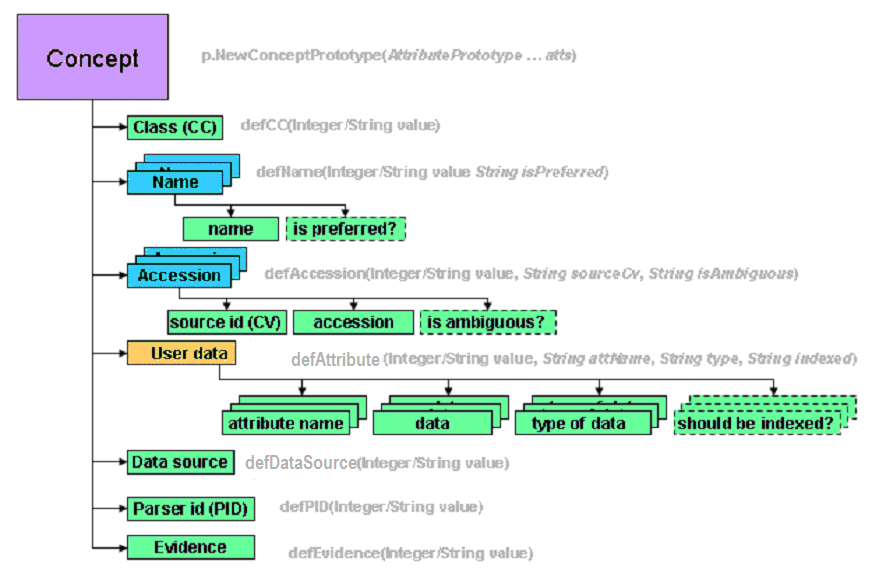
\includegraphics[scale=0.6]{images/Oct12/script_concept.png} 
\label{fig:script_concepts}
}
\subfigure[Data structure of an Ondex relation]{
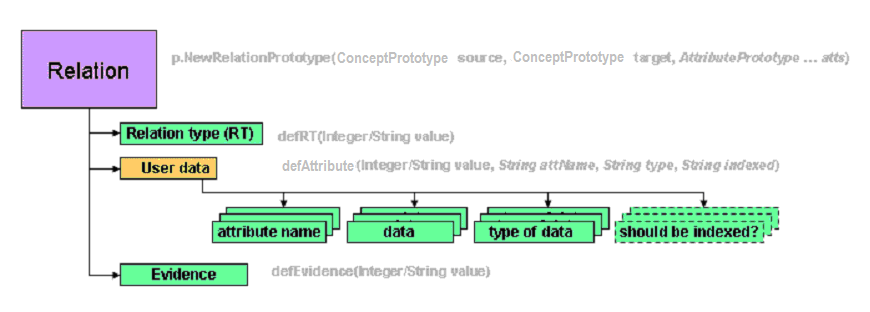
\includegraphics[scale=0.6]{images/Oct12/script_relation.png} 
\label{fig:script_relations}
}
\label{fig:script_concepts_relations}
\caption{Ondex data structure}
\end{figure}

\newpage
%%%%%%%%%%%%%%%%%%%%%%%%%%%%%%%%%%%%%%%%%%%%%%%%%%%%%%%%%%%%%%%%%%%%%%%%%%%%%%%%%%    
\section{Accession based mapping examples}
\label{sec:accmapping_examples}
This section illustrates how accession based mapping works with examples.

\subsection{No parameters}
\begin{center}
\begin{tabular}{|c|c|c|c|}\hline
Name & Concept Class & Data Source & Accession\\ \hline			
P1 & Protein & UNIPROTKB & UNIPROTKB:ACC1\\
P2 & Protein & TAIR & UNIPROTKB:ACC1\\
\hline  
\end{tabular}
\end{center}
\vspace{0.5cm}
P1 and P2 will map with no parameters needed because this mapping method maps concepts of the same concept class (Protein) and of different data source (UNIPROTKB and TAIR).

\subsection{EquivalentConceptClass parameter}
\begin{center}
\begin{tabular}{|c|c|c|c|}\hline
Name & Concept Class & Data Source & Accession\\ \hline			
P1 & Protein & UNIPROTKB & UNIPROTKB:ACC1\\
G1 & Gene & TAIR & UNIPROTKB:ACC1\\
\hline  
\end{tabular}
\end{center}
\vspace{0.5cm}
P1 and G1 will map if parameter EquivalentConceptClass is set to "Protein,Gene", so that the mapping method recognises these two concept classes as equivalent.

\subsection{EquivalentCV parameter (equivalent accession type)}
\begin{center}
\begin{tabular}{|c|c|c|c|}\hline
Name & Concept Class & Data Source & Accession\\ \hline			
P1 & Protein & UNIPROTKB & UNIPROTKB:ACC1\\
P2 & Protein & TAIR & TAIR:ACC1\\
\hline  
\end{tabular}
\end{center}
\vspace{0.5cm}
P1 and P2 will map if parameter EquivalentCV is set to "UNIPROTKB,TAIR", so that the mapping method recognises these two accession types as equivalent.

\subsection{WithinCVMapping parameter (within data source)}
\begin{center}
\begin{tabular}{|c|c|c|c|}\hline
Name & Concept Class & Data Source & Accession\\ \hline			
P1 & Protein & UNIPROTKB & UNIPROTKB:ACC1\\
P2 & Protein & UNIPROTKB & UNIPROTKB:ACC1\\
\hline  
\end{tabular}
\end{center}
\vspace{0.5cm}
P1 and P2 will map if parameter WithinCVMapping is set to true, so that the method maps concepts of the same concept class and same data source.

\subsection{IgnoreAmbiguity parameter (use ambiguous accessions)}
\begin{center}
\begin{tabular}{|c|c|c|c|c|}\hline
Name & Concept Class & Data Source & Accession & Ambiguous\\ \hline			
P1 & Protein & UNIPROTKB & UNIPROTKB:ACC1 & false\\
P2 & Protein & TAIR & UNIPROTKB:ACC1 & true\\
\hline  
\end{tabular}
\end{center}
\vspace{0.5cm}
P1 and P2 will map if the parameter IgnoreAmbiguity is set to true, so that the mapping method ignores the P2's ambiguous flag.

\subsection{ConceptClassRestriction parameter}
\begin{center}
\begin{tabular}{|c|c|c|c|}\hline
Name & Concept Class & Data Source & Accession\\ \hline			
P1 & Protein & UNIPROTKB & UNIPROTKB:ACC1\\
P2 & Protein & TAIR & UNIPROTKB:ACC1\\
G1 & Gene & UNIPROTKB & UNIPROTKB:ACC1\\
G2 & Gene & TAIR & UNIPROTKB:ACC1\\
\hline  
\end{tabular}
\end{center}
\vspace{0.5cm}
If no parameters are specified, two relations will be created: one between the two genes and one between the two proteins.
If the parameter ConceptClassRestriction is set to Protein, only the two proteins will be mapped.

\subsection{CVRestriction parameter (accession type restriction)} 
\begin{center}
\begin{tabular}{|c|c|c|c|}\hline
Name & Concept Class & Data Source & Accession\\ \hline			
P1 & Protein & UNIPROTKB & UNIPROTKB:ACC1\\
P2 & Protein & UNIPROTKB & TAIR:ACC1\\
P3 & Protein & TAIR & UNIPROTKB:ACC1\\
P4 & Protein & TAIR & TAIR:ACC1\\
\hline  
\end{tabular}
\end{center}
\vspace{0.5cm}
If no parameters are specified, two relations will be created: one between P1 and P3, and one between P2 and P4.
If the parameter CVrestriction is set to TAIR, only P2 and P4 will be mapped.

\subsection{WithinCVMapping parameter (within data source) and EquivalentCV parameter (equivalent accession type)} 
\begin{center}
\begin{tabular}{|c|c|c|c|}\hline
Name & Concept Class & Data Source & Accession\\ \hline			
P1 & Protein & UNIPROTKB & UNIPROTKB:ACC1\\
P2 & Protein & UNIPROTKB & TAIR:ACC1\\
\hline  
\end{tabular}
\end{center}
\vspace{0.5cm}
P1 and P2 will be mapped if WithinCVMapping is set to true and EquivalentCV is set to "UNIPROTKB,TAIR".


%%%%%%%%%%%%%%%%%%%%%%%%%%%%%%%%%%%%%%%%%%%%%%%%%%%%%%%%%%%%%%%%%%%%%%%%%%%%%%%%%%    
\section{Exercise}
Open file Tutorial\_files/Data\_integration/Exercise/exercise.tab in a text editor.
\subsection{Scripting Console}
\begin{itemize}
\item Edit Data\_integration/Exercise/exercise\_scripting.txt to import the 6 concepts in exercise.tab in Ondex using the scripting console.
As Section \ref{sec:parsing_tabdel} showed, the scripting console maps equivalent concepts by default and collapses them. 
For the purpose of the following exercise, exercise\_scripting.txt contains a p.setProcessingOptions() command which disables this feature.
Please use "UNIPROTKB" whenever defining "defAccession".
\item Once the scripting console has generated six concepts, save your graph.
\end{itemize}

\subsection{Integrator}
\begin{itemize}
\item Open the integrator and compose a workflow to import the graph you have just saved, 
map concepts based on their accessions (with no parameters for now) and export. 
\item Before opening your resulting graph, guess which concepts have been mapped and are now linked by new relations.
\item Come back to your workflow and experiment with parameters aiming to map:
	\begin{itemize}
	\item P2 and P4
	\item P3 and G2
	\item P1 and G1
	\end{itemize}
Do other concepts map too? Why?	
\end{itemize}

